\documentclass{standalone}
%
\usepackage{tikz}
\usetikzlibrary{backgrounds,arrows.meta,shapes.callouts}
\usepackage{xcolor}
%
\definecolor{space}{HTML}{1F2C4E}
\definecolor{earth}{HTML}{0089FA}
\definecolor{dida}{HTML}{FFDE00}
\definecolor{title}{HTML}{FBA706}
\definecolor{galaxy}{HTML}{4278A4}
\definecolor{paper01}{HTML}{BE8A3F}
\definecolor{paper02}{HTML}{E5D09B}
%
\usepackage{fontspec}
\setmainfont{Open Dyslexic}
%
\title{Vite nascoste}
\begin{document}
	\begin{tikzpicture}[background rectangle/.style={fill=white},show background rectangle,>={[inset=0,angle'=27]Stealth}]
		% title
		\draw [black,ultra thick,fill=title] (0,12.8) rectangle (30,16.8);
		\node at (15,14.8) {\textcolor{black}{\fontsize{75}{76}\selectfont Vite nascoste}};
		% stripe
		\begin{scope}[shift={(0,12)}]
			\draw [fill=earth!50!white, thick] (14.5,0) rectangle (26.5,-130.5);
			\foreach \i in {0,1,...,11}
			{
				\draw [fill=white, thick] (14.75+\i,-0.5) rectangle (15.25+\i,-1);
			}
			%
			\foreach \j in {0,1,...,11}
			{
				\draw [fill=white, thick] (14.75+\j,-128.5) rectangle (15.25+\j,-129);
			}
		\end{scope}
		%
		% Katherine Johnson
		%
		\begin{scope}[shift={(0,8)}]
			\draw [fill=earth!50!space, thick] (3,1.35) rectangle (13,-11.35);
			\node at (8,-5) {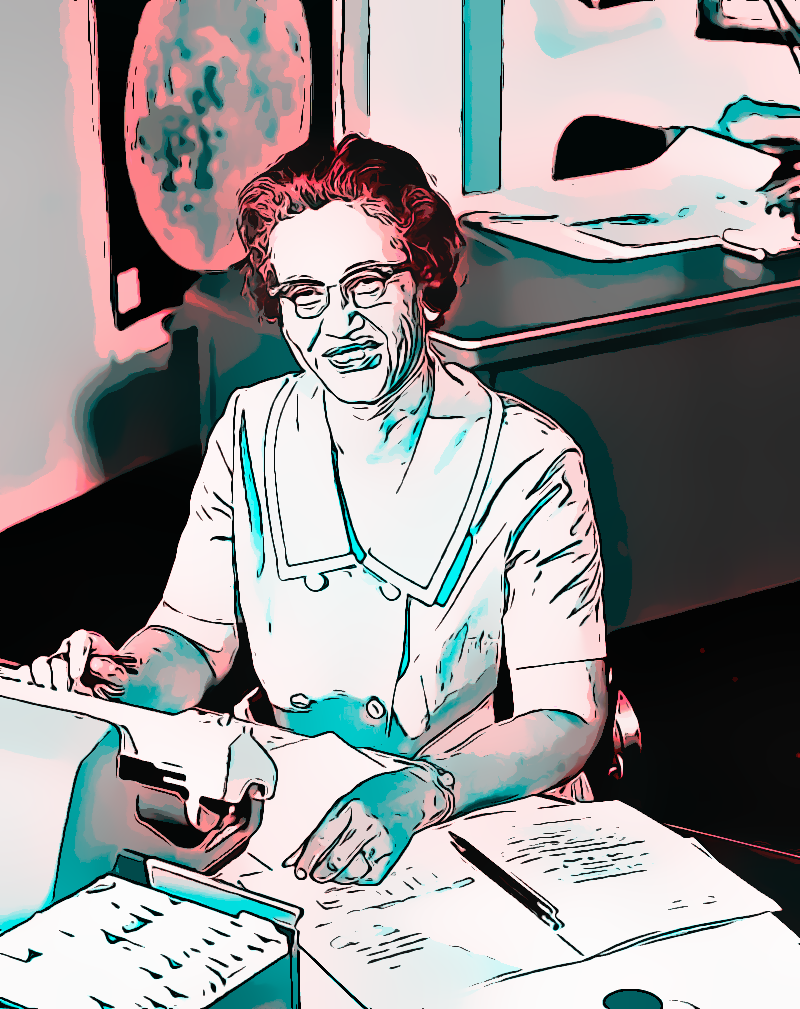
\includegraphics[width=10cm]{img/2023/katherine_johnson}};
			%
			\draw [fill=galaxy, ultra thick] (4.6,-10.8) rectangle (11.4,-11.9);
			\node at (8,-11.4) {\textcolor{black}{\fontsize{18}{19}\selectfont Katherine Johnson}};
			%
			\draw [fill=title, thick] (14,0.9) rectangle (27,1.8);
			\node (example-textwidth-2) [right, align=left, text width=12cm, color=black, font=\fontsize{18pt}{19pt}\selectfont] at (15,1.3) {\textbf{26 agosto 1918}};
			%
			\node (example-textwidth-2) [right, align=left, text width=12cm, color=black, font=\fontsize{18pt}{19pt}\selectfont] at (15,-0.1) {Matematica e astrofisica};
			%
			\shade [bottom color=paper02,top color=paper01]	(14,-1.1) rectangle (27,-21.3);
			\draw [thick] (14,-1.1) rectangle (27,-21.3);
			\node (example-textwidth-2) [right, align=left, text width=11cm, color=black, font=\fontsize{18pt}{19pt}\selectfont] at (15,-11.2) {\emph{Avevamo bisogno di essere assertive come donne, in quei giorni, assertive e aggressive, e il livello con cui dovevi esserlo dipendeva dal dove eri. Io dovevo esserlo. Nei primi giorni della NASA alle donne non era consentito mettere i loro nomi sui report - nessuna donna nel mio dipartimento ha avuto il suo nome su un report. Stavo lavorando con Ted Skopinski e voleva mollare e andare a Houston (...) ma Henry Pearson, il nostro supervisore - non era un sostenitore delle donne - continuava a spingerlo a finire il report su cui stavamo lavorando. Alla fine Ted gli disse: "Katherine dovrebbe finire il report, ha comunque fatto la maggior parte del lavoro". Così Ted lasciò Pearson senza alcuna scelta; finii il report e il mio nome venne messo su di esso, e quella fu la prima volta che una donna nel nostro dipartimento ebbe il suo nome su qualcosa.}};
			%
			\draw [fill=dida, thick] (14,-22) rectangle (27,-28);
			\node (example-textwidth-2) [right, align=left, text width=10cm, color=black, font=\fontsize{18pt}{19pt}\selectfont] at (15,-25) {Questo \emph{report}, scritto insieme con \textbf{Ted Skopinski}, contiene la teoria necessaria per il lancio, il traccamento e il rientro dei veicoli nello spazio. Fu fondamentale per le missioni di \textbf{Alan Shepard} e \textbf{John Glenn}.};
			%
			\node (example-textwidth-2) [right, align=left, text width=11cm, color=black, font=\fontsize{18pt}{19pt}\selectfont] at (15,-30) {Il \textbf{16 novembre del 2015} ha ricevuto la \emph{Presidential Medal of Freedom} dalle mani dell'allora presidente \textbf{Barack Obama}.};
			%
			\draw [fill=title, thick] (14,-31.8) rectangle (27,-32.8);
			\node (example-textwidth-2) [right, align=left, text width=12cm, color=black, font=\fontsize{18pt}{19pt}\selectfont] at (15,-32.3) {\textbf{24 febbraio 2020}};
		\end{scope}
		%
		% Dorothy Vaughan
		%
		\begin{scope}[shift={(0,-35.5)}]
			\foreach \i in {0,1,...,11}
			{
				\draw [fill=white, thick] (14.75+\i,9) rectangle (15.25+\i,9.5);
			}
			%
			\draw [fill=earth!50!white, thick] (3,6.85) rectangle (13,-6.85);
			\node at (8,0) {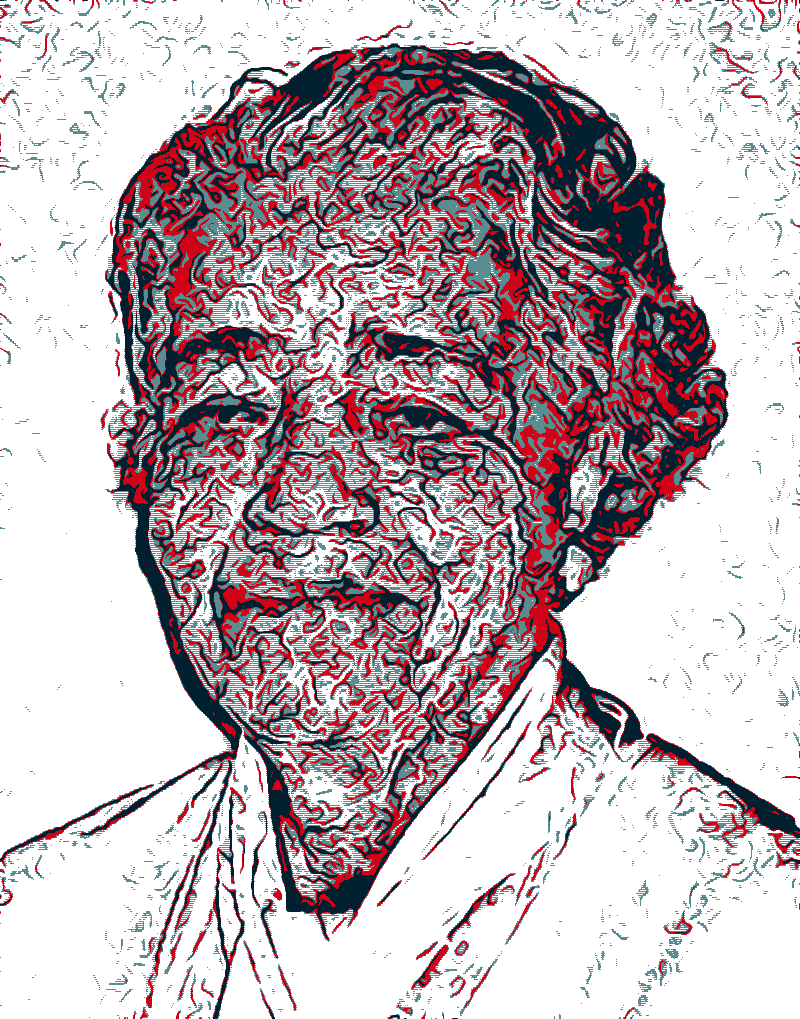
\includegraphics[width=10cm]{img/2023/dorothy_vaughan}};
			%
			\draw [fill=galaxy, ultra thick] (4.6,-6.5) rectangle (11.4,-7.5);
			\node at (8,-7) {\textcolor{black}{\fontsize{18}{19}\selectfont Dorothy Vaughan}};
			%
			\draw [fill=title, thick] (14,6.85) rectangle (27,7.75);
			\node (example-textwidth-2) [right, align=left, text width=12cm, color=black, font=\fontsize{18pt}{19pt}\selectfont] at (15,7.35) {\textbf{20 settembre 1910}};
			%
			\node (example-textwidth-2) [right, align=left, text width=12cm, color=black, font=\fontsize{18pt}{19pt}\selectfont] at (15,6) {Matematica e programmatrice};
			%
			\draw [fill=dida, thick] (14,5.4) rectangle (27,1.6);
			\node (example-textwidth-2) [right, align=left, text width=10cm, color=black, font=\fontsize{18pt}{19pt}\selectfont] at (15,3.5) {Si laurea a 19 anni in matematica presso la \emph{Wilberforce University}, storica università per afroamericani dell'Ohio.};
			%			%
			\node (example-textwidth-2) [right, align=left, text width=10cm, color=black, font=\fontsize{18pt}{19pt}\selectfont] at (15,-2.8) {Nel 1943, dopo 14 anni di insegnamento, iniziò a lavorare presso il \emph{Langley Memorial Aeronautical Laboratory} per poter fornire il suo contributo durante la seconda guerra mondiale. Pensava sarebbe stato un lavoro temporaneo. E invece la tenne occupata per i 28 anni successivi.};
			%
			\draw [fill=dida, thick] (14,-7) rectangle (27,-15);
			\node (example-textwidth-2) [right, align=left, text width=11cm, color=black, font=\fontsize{18pt}{19pt}\selectfont] at (15,-11) {Dopo la trasformazione della NACA alla NASA, passò alla \emph{Analysis and Computation Division}, un gruppo misto di calcolatori di ogni genere e razza. Qui divenne un'esperta di \textbf{FORTRAN}, sviluppando i programmi che avrebbero permesso di calcolare le traiettorie dei razzi lanciati verso lo spazio.};
			%
			\draw [fill=title, thick] (14,-15.6) rectangle (27,-16.6);
			\node (example-textwidth-2) [right, align=left, text width=12cm, color=black, font=\fontsize{18pt}{19pt}\selectfont] at (15,-16) {\textbf{10 novembre 1951}};
		\end{scope}
		%
		% Mary Jackson
		%
		\begin{scope}[shift={(0,-62.7)}]
			\foreach \i in {0,1,...,11}
			{
				\draw [fill=white, thick] (14.75+\i,8.8) rectangle (15.25+\i,9.3);
			}
			%
			\draw [thick] (3,6.55) rectangle (13,-1.55);
			\node at (8,2.5) {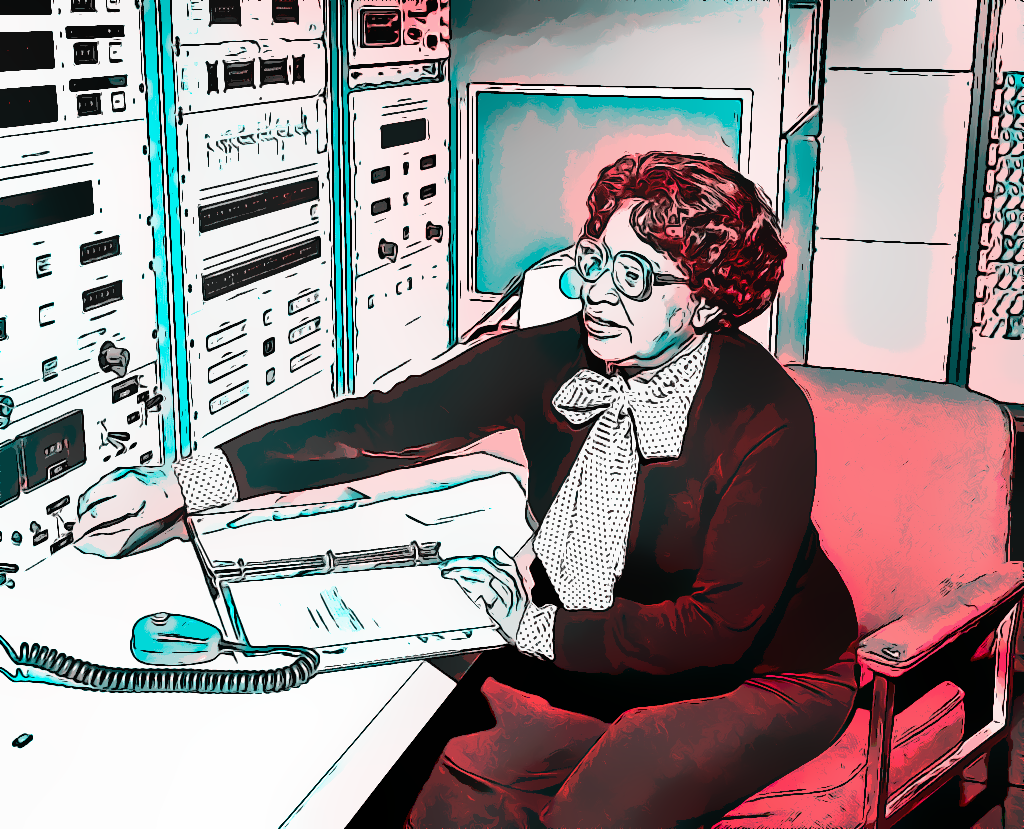
\includegraphics[width=10cm]{img/2023/mary_jackson}};
			%
			\draw [fill=galaxy, ultra thick] (5.3,-1.1) rectangle (10.7,-2.1);
			\node at (8,-1.6) {\textcolor{black}{\fontsize{18}{19}\selectfont Mary Jackson}};
			%
			\draw [fill=title, thick] (14,6.55) rectangle (27,7.45);
			\node (example-textwidth-2) [right, align=left, text width=12cm, color=black, font=\fontsize{18pt}{19pt}\selectfont] at (15,6.95) {\textbf{9 aprile 1921}};
			%
			\node (example-textwidth-2) [right, align=left, text width=10cm, color=black, font=\fontsize{18pt}{19pt}\selectfont] at (15,5.6) {Ingegnere};
			%
			\draw [fill=dida, thick] (14,-1.8) rectangle (27,4.8);
			\node (example-textwidth-2) [right, align=left, text width=10cm, color=black, font=\fontsize{18pt}{19pt}\selectfont] at (15,1.5) {Forte di una laurea in matematica e fisica ottenuta presso la \emph{Hampton University} nel 1942, nel 1951 inizia a lavorare presso il \emph{Langley Research Center} come calcolatrice sotto la supervisione di \textbf{Dorothy Vaughan}.};
			%
			\node (example-textwidth-2) [right, align=left, text width=11cm, color=black, font=\fontsize{18pt}{19pt}\selectfont] at (15,-5.3) {A partire dal 1953 iniziò a lavorare presso il Supersonic Pressure Tunnel insieme con l'ingegnere \textbf{Kazimierz Czarnecki}. Quest'ultimo la incoraggiò seguire i corsi necessari per ottenere la laurea in ingegneria. Cosa che riuscì a fare, non senza qualche difficoltà.};			
			%
			\draw [fill=dida, thick] (14,-9) rectangle (27,-14.4);
			\node (example-textwidth-2) [right, align=left, text width=11cm, color=black, font=\fontsize{18pt}{19pt}\selectfont] at (15,-11.7) {E' diventata la prima donna ingnegnere della NASA, occupandosi in particolare dello studio dei flussi dell'aria, comprese le forze di spinta e d'attrito, in modo da migliorare la costruzione degli aereoplani.};
			%
			\node (example-textwidth-2) [right, align=left, text width=11cm, color=black, font=\fontsize{18pt}{19pt}\selectfont] at (15,-16.3) {Ottenuto il ruolo di \emph{senior engeenering} nel 1979, ha deciso di impegnarsi sempre di più nel campo delle pari opportunità.};
			%
			\draw [fill=title, thick] (14,-18.3) rectangle (27,-19.2);
			\node (example-textwidth-2) [right, align=left, text width=12cm, color=black, font=\fontsize{18pt}{19pt}\selectfont] at (15,-18.8) {\textbf{11 febbraio 2005}};
		\end{scope}
		%
		% Evelyn Boyd
		%
		\begin{scope}[shift={(0,-89.5)}]
			\foreach \i in {0,1,...,11}
			{
				\draw [fill=white, thick] (14.75+\i,6.4) rectangle (15.25+\i,5.9);
			}
			%
			\draw [thick] (3,3.95) rectangle (13,-6.45);
			\node at (8,-1.25) {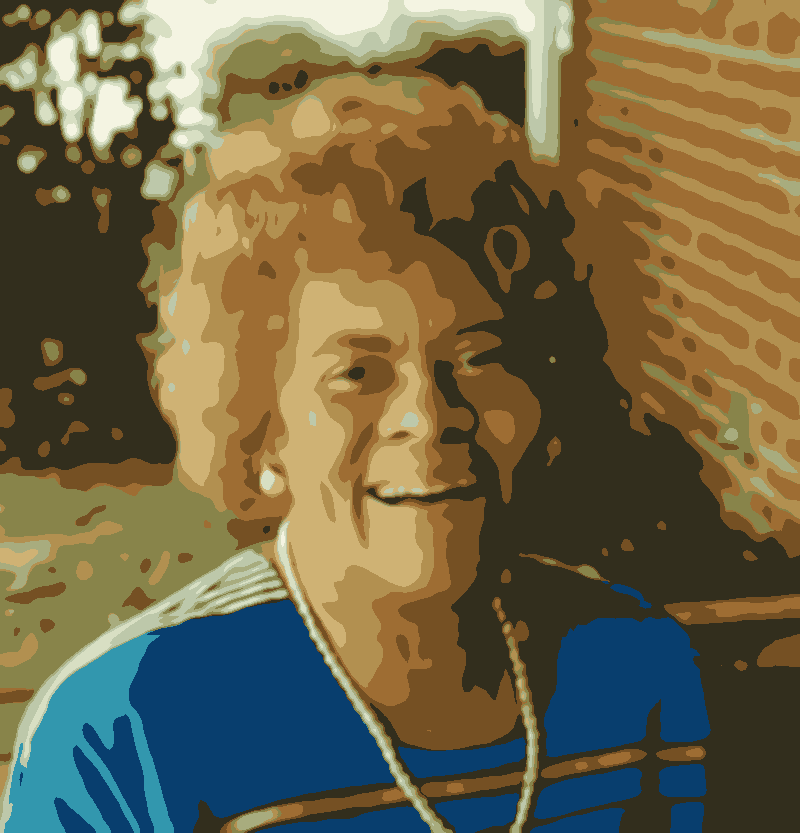
\includegraphics[width=10cm]{img/2023/evelyn_boyd}};
			%
			\draw [fill=galaxy, ultra thick] (5.6,-6) rectangle (10.4,-7);
			\node at (8,-6.5) {\textcolor{black}{\fontsize{18}{19}\selectfont Evelyn Boyd}};
			%
			\draw [fill=title, thick] (14,3.95) rectangle (27,4.85);
			\node (example-textwidth-2) [right, align=left, text width=12cm, color=black, font=\fontsize{18pt}{19pt}\selectfont] at (15,4.35) {\textbf{1 maggio 1924}};
			%
			\node (example-textwidth-2) [right, align=left, text width=10cm, color=black, font=\fontsize{18pt}{19pt}\selectfont] at (15,3) {Matematica};
			%
			\shade [bottom color=paper02,top color=paper01] (14,2.2) rectangle (27,-7.6);
			\draw [thick] (14,2.2) rectangle (27,-7.6);
			\node (example-textwidth-2) [right, align=left, text width=11cm, color=black, font=\fontsize{18pt}{19pt}\selectfont] at (14.8,-2.7) {\emph{Ero affascinata dallo studio dell'astronomia e ad un certo punto mi gingillai con l'idea di spostare la mia attenzione a questa materia. Se avessi saputo che in un futuro non così distante gli Stati Uniti avrebbero lanciato il loro programma spaziale, e che gli astronomi sarebbero stati molto richiesti per la plianificazione delle missioni spaziali, avrei potuto diventare un'astronoma invece che una matematica.}};
			%
			\node (example-textwidth-2) [right, align=left, text width=12cm, color=black, font=\fontsize{18pt}{19pt}\selectfont] at (15,-11.7) {Nel 1960 iniziò a lavorare a Los Angeles, presso gli \emph{US Space Technology Laboratories}, che nel 1962 divennero la \emph{North American Aviation Space and Information Systems Division}. In questa sede contribuì a vari progetti collegati al \emph{programma Apollo} relativi alla meccanica celeste, al calcolo delle traiettorie e allo sviluppo di tecniche informatiche digitali.};
			%
			\draw [fill=dida, thick] (14,-15.7) rectangle (27,-25.7);
			\node (example-textwidth-2) [right, align=left, text width=12cm, color=black, font=\fontsize{18pt}{19pt}\selectfont] at (15,-20.7) {Nel 1951, insieme con due colleghi afro-americani, le venne negato l'accesso a un incontro regionale della \emph{Mathematical Association of America} (MAA), perché si svolgeva presso un hotel riservato ai bianchi. Come conseguenza di questo increscioso episodio e sotto la pressione di \textbf{Lee Lorch}, matematico, attivista per i diritti civili e comunista, l'MAA e la \emph{American Mathematical Society} (AMS) modificarono le loro regole per migliorare l'inclusione.};
		\end{scope}
		% image credits
		\begin{scope}[shift={(0,-120)}]
			\draw [fill=space,thick] (2,1) rectangle (28,-1);
			%
			\node (example-textwidth-2) [right, align=left, text width=25cm, color=white, font=\fontsize{18pt}{19pt}\selectfont] at (2.5,0) {Le immagini sono tratte da Wikipedia o dalla NASA e poi rielaborate graficamente usando il filtro G'MIC-Qt di Gimp.};
		\end{scope}
		%
		\begin{scope}[shift={(0,-122)}]
			\node at (27,0) () {
\includegraphics[width=3.7cm]{licenza}};
			\node (example-textwidth-2) [right, align=left, text width=14cm, color=black, font=\fontsize{14pt}{15pt}\selectfont] at (12.5,-0.1) {Testo e grafica: @ulaulaman - Gianluigi Filippelli};
		\end{scope}
	\end{tikzpicture}
\end{document}
